\begin{tikzpicture}[
    scale=0.9,
    every node/.style={circle, draw, minimum size=7mm}
]

\tikzset{iso/.style={fill=#1, draw=black, text=white}}

% =========================================================
% ======================== G1 =============================
% =========================================================

% Coloration différente de la forme canonique
\node   (v1) at (0,2.5)   {$1$};
\node  (v2) at (-1.5,1)  {$2$};
\node (v3) at (1.5,1)   {$3$};
\node    (v4) at (-1,-0.5) {$4$};
\node   (v5) at (1,-0.5)  {$5$};
\node (v6) at (0,-2)    {$6$};
\node    (v7) at (0,0.5)   {$7$};

\draw (v1)--(v2);
\draw (v1)--(v3);
\draw (v2)--(v4);
\draw (v3)--(v5);
\draw (v4)--(v6);
\draw (v5)--(v6);
\draw (v4)--(v7);
\draw (v5)--(v7);
\draw (v6)--(v7);

\node[draw=none, rectangle] at (0,-2.7) {$G_1$};



% =========================================================
% ======================== G2 =============================
% =========================================================

% Coloration différente de G1
\node  (u1) at (6,2)      {$a$};
\node   (u2) at (8,1.5)    {$b$};
\node (u3) at (7,0)      {$c$};
\node    (u4) at (5.5,-0.5) {$d$};
\node   (u5) at (8,-1)     {$e$};
\node  (u6) at (6,-2)     {$f$};
\node    (u7) at (7,-1)     {$g$};

\draw (u1)--(u2);
\draw (u1)--(u4);
\draw (u2)--(u3);
\draw (u3)--(u5);
\draw (u4)--(u6);
\draw (u5)--(u6);
\draw (u4)--(u7);
\draw (u5)--(u7);
\draw (u6)--(u7);

\node[draw=none, rectangle] at (7,-2.7) {$G_2$};



% =========================================================
% ================= Symbole d'isomorphisme ===============
% =========================================================

\node[draw=none, rectangle] at (3.5,0.5) {\Large $\overset{?}{\cong}$};



% =========================================================
% ===================== Forme canonique ===================
% =========================================================

% Les deux graphes sont maintenant STRICTEMENT identiques

% ------------------------- G1 -----------------------------

\node[iso=red]     (v1c) at (0,-5.5)   {$1$};
\node[iso=blue]    (v2c) at (-1.5,-7)  {$2$};
\node[iso=orange]  (v3c) at (1.5,-7)   {$3$};
\node[iso=violet]  (v4c) at (-1,-8.5)  {$4$};
\node[iso=teal]    (v5c) at (1,-8.5)   {$5$};
\node[iso=brown]   (v6c) at (0,-10)    {$6$};
\node[iso=magenta] (v7c) at (0,-7.5)   {$7$};

\draw (v1c)--(v2c);
\draw (v1c)--(v3c);
\draw (v2c)--(v4c);
\draw (v3c)--(v5c);
\draw (v4c)--(v6c);
\draw (v5c)--(v6c);
\draw (v4c)--(v7c);
\draw (v5c)--(v7c);
\draw (v6c)--(v7c);

\node[draw=none, rectangle] at (0,-10.7) {$G_1^{\mathrm{can}}$};



% ------------------------- G2 -----------------------------



\begin{scope}[yshift=-7.5cm]
    \node[iso=blue]    (u1c) at (6,2)      {$a$};
    \node[iso=red]     (u2c) at (8,1.5)    {$b$};
    \node[iso=orange]  (u3c) at (7,0)      {$c$};
    \node[iso=violet]  (u4c) at (5.5,-0.5) {$d$};
    \node[iso=teal]    (u5c) at (8,-1)     {$e$};
    \node[iso=brown]   (u6c) at (6,-2)     {$f$};
    \node[iso=magenta] (u7c) at (7,-1)     {$g$};
  
    \draw (u1c)--(u2c);
    \draw (u1c)--(u4c);
    \draw (u2c)--(u3c);
    \draw (u3c)--(u5c);
    \draw (u4c)--(u6c);
    \draw (u5c)--(u6c);
    \draw (u4c)--(u7c);
    \draw (u5c)--(u7c);
    \draw (u6c)--(u7c);
  \end{scope}


\node[draw=none, rectangle] at (7,-10.7) {$G_2^{\mathrm{can}}$};


\node[draw=none, rectangle] at (3.5,-7.5) {\Large $\overset{?}{=}$};
% =========================================================
% ======================== Flèches ========================
% =========================================================

\draw[->, thick]
    (0,-3.0) -- (0,-4.8)
    node[midway, right=2mm, draw=none, rectangle] {\small forme canonique};

\draw[->, thick]
    (7,-3.0) -- (7,-4.8)
    node[midway, right=2mm, draw=none, rectangle] {\small forme canonique};

\end{tikzpicture}